\documentclass[12pt, titlepage]{article}

\usepackage{fullpage}
\usepackage[round]{natbib}
\usepackage{multirow}
\usepackage{booktabs}
\usepackage{tabularx}
\usepackage{graphicx}
\usepackage{float}
\usepackage{hyperref}
\usepackage{float}
\usepackage[letterpaper, portrait, margin=1in]{geometry}
\usepackage{helvet}
\hypersetup{
    colorlinks,
    citecolor=blue,
    filecolor=black,
    linkcolor=red,
    urlcolor=blue
}

\usepackage{afterpage}
\usepackage{titlepic}
\usepackage[dvipsnames]{xcolor}

\usepackage{titlesec}
\titleformat{\section}{\large\bfseries\color{RedOrange}}{\rlap{\color{black}\rule[-0.3cm]{\linewidth}{1cm}} {\textcolor{RedOrange}{\thesection}}}{1em}{}


\renewcommand{\familydefault}{\sfdefault}
%% Comments

\usepackage{color}

\newif\ifcomments\commentstrue %displays comments
%\newif\ifcomments\commentsfalse %so that comments do not display

\ifcomments
\newcommand{\authornote}[3]{\textcolor{#1}{[#3 ---#2]}}
\newcommand{\todo}[1]{\textcolor{red}{[TODO: #1]}}
\else
\newcommand{\authornote}[3]{}
\newcommand{\todo}[1]{}
\fi

\newcommand{\wss}[1]{\authornote{blue}{SS}{#1}} 
\newcommand{\plt}[1]{\authornote{magenta}{TPLT}{#1}} %For explanation of the template
\newcommand{\an}[1]{\authornote{cyan}{Author}{#1}}

%% Common Parts

\newcommand{\progname}{ProgName} % PUT YOUR PROGRAM NAME HERE
\newcommand{\authname}{Team \#, Team Name
\\ Student 1 name and macid
\\ Student 2 name and macid
\\ Student 3 name and macid
\\ Student 4 name and macid} % AUTHOR NAMES                  

\usepackage{hyperref}
    \hypersetup{colorlinks=true, linkcolor=blue, citecolor=blue, filecolor=blue,
                urlcolor=blue, unicode=false}
    \urlstyle{same}
                                


\newcounter{acnum}
\newcommand{\actheacnum}{AC\theacnum}
\newcommand{\acref}[1]{AC\ref{#1}}

\newcounter{ucnum}
\newcommand{\uctheucnum}{UC\theucnum}
\newcommand{\uref}[1]{UC\ref{#1}}

\newcounter{mnum}
\newcommand{\mthemnum}{M\themnum}
\newcommand{\mref}[1]{M\ref{#1}}

\begin{document}

\title{\textbf{System Design for \progname{}} \\ \vspace{2cm} 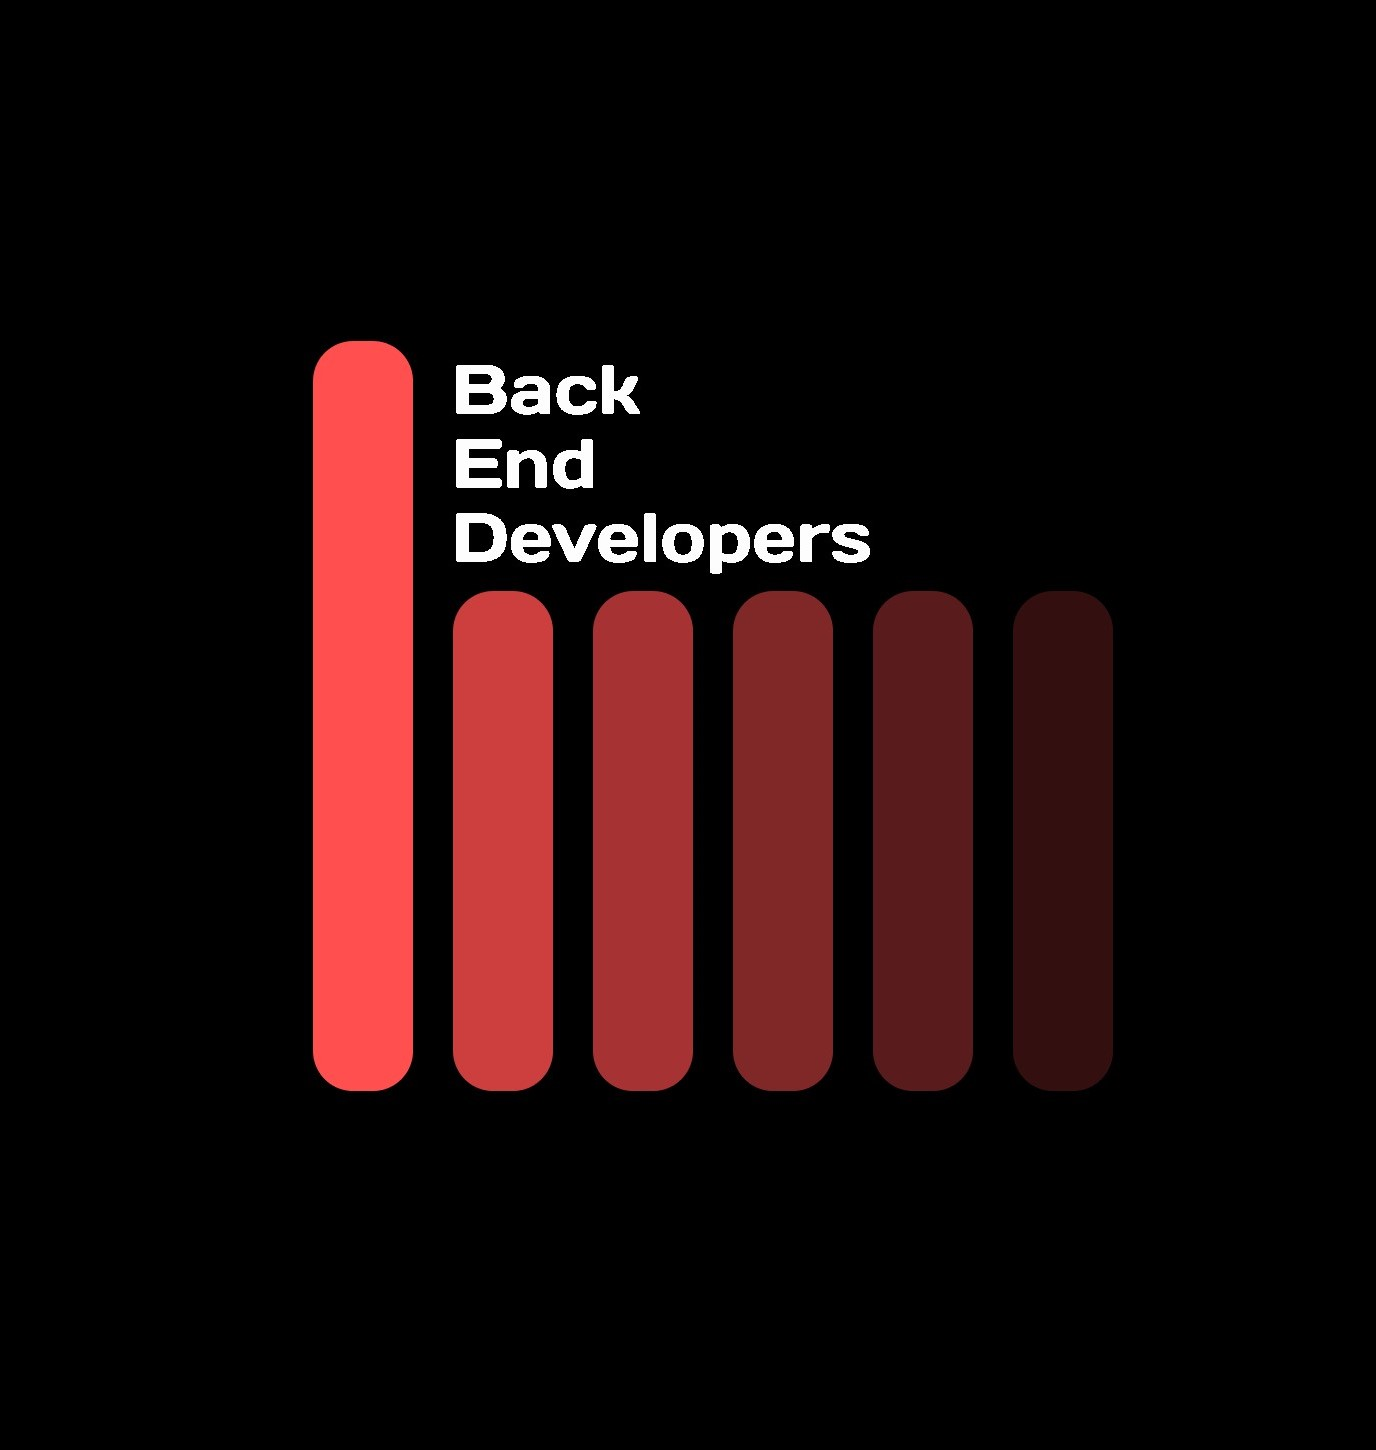
\includegraphics[width=0.5\textwidth]{../../logo.jpg}}
 \pagecolor{black}\afterpage{\nopagecolor}
\author{\authname}
\date{\today}

\color{white}\maketitle
\color{black}
\pagenumbering{roman}

\section{Revision History}

\begin{tabularx}{\textwidth}{p{4cm}p{2cm}X}
\toprule {\bf Date} & {\bf Version} & {\bf Notes}\\
\midrule
2023-01-18 & 1.0 & Initial documentation\\
2023-03-15 & 2.0 & Modified and proofread for Revision 1 \\
2023-03-25 & 2.1 & Incorporated TA feedback \\
2023-04-04 & 2.2 & Added logo and style to the document \\
\bottomrule
\end{tabularx}

\newpage

\section{Reference Material}

This section records information for easy reference.

\subsection{Abbreviations and Acronyms}
Refer to \href{https://github.com/zakerl/Capstone_Project/blob/main/docs/SRS/SRS.pdf}{SRS} for a comprehensive list of abbreviations and acronyms.\\

\renewcommand{\arraystretch}{1.2}
\begin{tabular}{l l} 
  \toprule		
  \textbf{symbol} & \textbf{description}\\
  \midrule 
	Lipo battery & Lithium polymer battery\\
	PCB & Printed circuit board\\
	TFT LCD Display & Thin film transistor liquid crystal display\\
	FSM & Finite state machine\\
	UI & User interface\\
	CAD & Computer aided design for 3D models\\
	SPI & Serial peripheral interface\\

  \bottomrule
\end{tabular}\\


\newpage

\tableofcontents

\newpage

\listoftables

\listoffigures

\newpage

\pagenumbering{arabic}

\section{Introduction}

This document provides a detailed description of the system design for the EMAnator; the system currently under development by the Back End Developers which aims to assist researchers in performing Ecological Momentary Assessment for older adults. The goal of this design is to construct a system which fulfills all the requirements specified in the \href{https://github.com/zakerl/Capstone_Project/blob/desDoc_Labeeb/docs/SRS/SRS.pdf}{System Requirements Specification}, and that meets the needs of EMA researchers.\\

This document provides the big-picture goals of the system, an overview of the project, a comprehensive list of system variables, and details regarding the user interfaces of the system. It also lists the various hardware and electrical components involved in the design of the system. Finally, it includes a high-level timeline for the development of the system. \\

The design presented in this document is the result of collaboration between the Dr. Luciana Macedo of the School of Rehabilitative Sciences and the Back End Developers development team. We have discussed the project requirements and identified the best approach to meet them. This is covered in detail in the document titled \href{https://github.com/zakerl/Capstone_Project/blob/desDoc_Labeeb/docs/ProblemStatementAndGoals/Team1_ProblemStatement\%20\%26\%20Goals.pdf}{Problem Statement and Goals}.\\

The Back End Developers hope this document serves as a useful guide for anyone involved in the development or deployment of the system. \\


\section{Purpose}

In general, engineering design documentation is a set of documents that outline the detailed specifications for an engineering project. It describes the design of the project, including its requirements, the materials to be used, the processes involved, the safety and environmental considerations, and the estimated costs. The purpose of engineering design documentation is to provide a comprehensive record of the project that can be consulted by engineers, oversight bodies, and other stakeholders throughout the project’s life cycle.\\

This documentation includes technical drawings, process diagrams, system and component specifications, and relevant schematics and images. It also provides a basis for quality control and assurance, as well as a way to track progress and identify potential areas of improvement. It is an essential part of any engineering project, as it ensures that all stakeholders have a clear understanding of the project and the necessary steps for its successful completion.\\
\newpage
This project currently has the current pieces of design documentation available:

\begin{itemize}
	\item \href{https://github.com/zakerl/Capstone_Project/blob/main/docs/ProblemStatementAndGoals/Team1_ProblemStatement\%20\%26\%20Goals.pdf}{Problem Statment and Goals}
	\item \href{https://github.com/zakerl/Capstone_Project/blob/main/docs/DevelopmentPlan/DevelopmentPlan.pdf}{Development Plan}
	\item \href{https://github.com/zakerl/Capstone_Project/blob/main/docs/SRS/SRS.pdf}{System Requirements Specification}
	\item \href{https://github.com/zakerl/Capstone_Project/blob/main/docs/HazardAnalysis/HazardAnalysis.pdf}{Hazard Analysis}
	\item \href{https://github.com/zakerl/Capstone_Project/blob/main/docs/VnVPlan/VnVPlan.pdf}{VnV Plan}
	\item \href{https://github.com/zakerl/Capstone_Project/blob/main/docs/Design/SoftArchitecture/MG.pdf}{Module Guide}
	\item \href{https://github.com/zakerl/Capstone_Project/blob/main/docs/Design/SoftDetailedDes/MIS.pdf}{Module Interface Specification}
\end{itemize}

\section{Scope}

This system in theory is very simple. An array of sensors grabs info regarding the position, speed, orientation, etc. and uses that information to understand the current state of the user. This data is then used to generate prompts that the user will answer and all the collected data is compiled, processed and stored within the system. Finally, researchers will analyze the collected data and generate observations. \\

\begin{figure}[H]
\begin{center}
 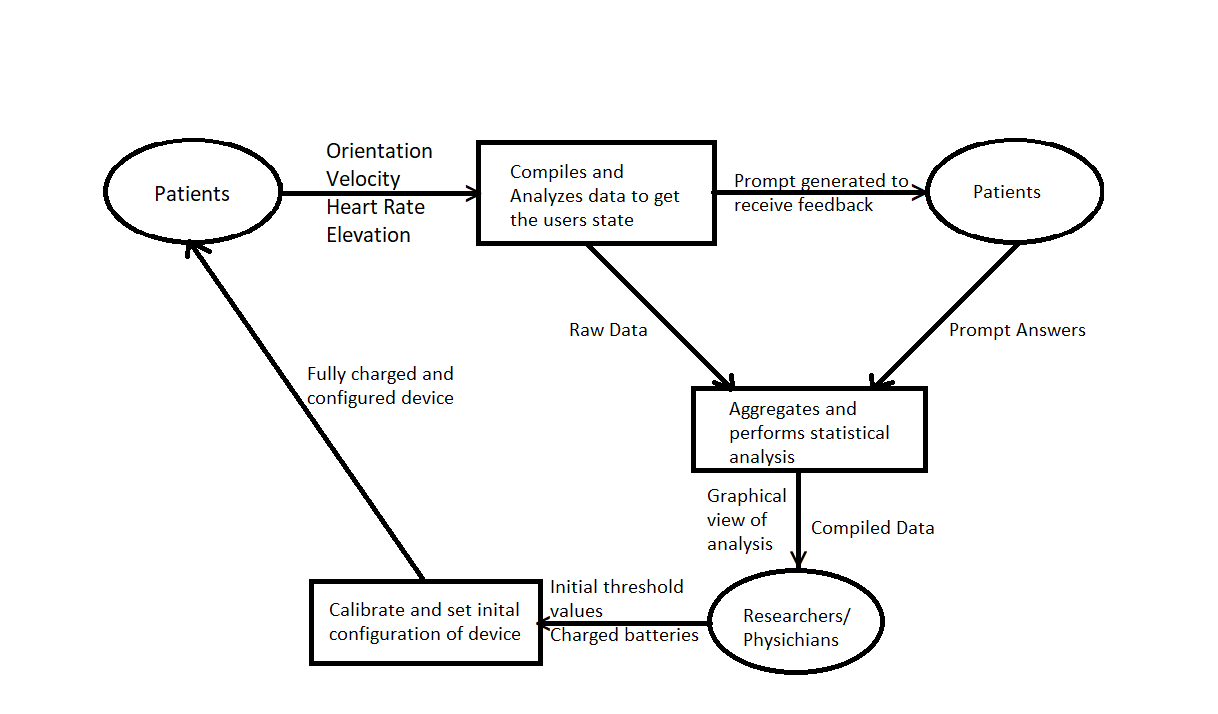
\includegraphics[width=.95\textwidth]{System Context Diagram}
\caption{System Context}
\label{Fig_SystemContext} 
\end{center}
\end{figure}

\section{Project Overview}

\subsection{Normal Behaviour}

Refer to \href{https://github.com/zakerl/Capstone_Project/blob/main/docs/SRS/SRS.pdf}{SRS} Section 12.

\subsection{Undesired Event Handling}

Refer to \href{https://github.com/zakerl/Capstone_Project/blob/main/docs/SRS/SRS.pdf}{SRS} Section 13.

\subsection{Component Diagram}

Refer to Section \ref{dEC}

\subsection{Connection Between Requirements and Design} \label{SecConnection}

\begin{table}[H]
	\begin{tabular}{|p{3cm} | p{12cm}| }
		 \hline
		 \textbf{Requirement} & \textbf{Deisgn Decisions} \\
		\hline
		R\href{https://github.com/zakerl/Capstone_Project/blob/main/docs/SRS/SRS.pdf}{1}  & The user will be reminded to charge the device during their introduction to the device and a LiPo for longer battery life. \\		 
		\hline
		R\href{https://github.com/zakerl/Capstone_Project/blob/main/docs/SRS/SRS.pdf}{2} & The device integrates the heartrate sensor and the MPU accelerometer on the same PCB. Using them together in a sensor array module minor movements of the user can be tracked and then stored in the database. \\
		\hline
		 R\href{https://github.com/zakerl/Capstone_Project/blob/main/docs/SRS/SRS.pdf}{3} & Using the same sensor integration above the user is prompted based on researcher defined thresholds on initial device setup which is done in the local GUI. \\
		\hline
		R\href{https://github.com/zakerl/Capstone_Project/blob/main/docs/SRS/SRS.pdf}{4} & The device is in the form of a smartwatch. It is lightweight and intuitive for the user. \\
		\hline
		R\href{https://github.com/zakerl/Capstone_Project/blob/main/docs/SRS/SRS.pdf}{5} & In the local user interface, the researcher is able to configure thresholds for the input parameters that can be customized for each user. \\
		 \hline
		R\href{https://github.com/zakerl/Capstone_Project/blob/main/docs/SRS/SRS.pdf}{6}  & Using the SD card reader module data is stored when a user completes the EMA which is prompted on the watch display. \\
		\hline 
		 R\href{https://github.com/zakerl/Capstone_Project/blob/main/docs/SRS/SRS.pdf}{7}& Using the device manager module and the SD card module data can be extracted and read locally by the researcher. Once read using the grapical plotter module the data can be analyzed in graphical format or extracted in raw format through an encrypted *.csv file. \\
		\hline
	\end{tabular}
\caption{\label{Hardware User Interface}Components of Hardware UI}  
\end{table}

\section{System Variables}

\subsection{Monitored Variables}

Refer to \href{https://github.com/zakerl/Capstone_Project/blob/main/docs/SRS/SRS.pdf}{SRS} Section 5.1.2.
\subsection{Controlled Variables}

Refer to \href{https://github.com/zakerl/Capstone_Project/blob/main/docs/SRS/SRS.pdf}{SRS} Section 5.1.3.

\subsection{Constants Variables}

Refer to \href{https://github.com/zakerl/Capstone_Project/blob/main/docs/SRS/SRS.pdf}{SRS} Section 1.4.
\section{User Interfaces}


\subsection{Hardware User Interface}

The device is worn by a participant on the wrist for measuring activity and generating  prompts. The following items will be shown on the display of the activity tracker:
\begin{table}[H]
	\begin{tabularx}{1.05\textwidth} { 
		  | >{\centering\arraybackslash}X 
		  | >{\centering\arraybackslash}X 
		  | >{\centering\arraybackslash}X 
		  | >{\centering\arraybackslash}X | }
		 \hline
		 \textbf{Description} & \textbf{Behaviour of TFT Display} \\
		 \hline
		Power up of activity tracker. & Displays Back End Developers on startup.\\
		\hline
		 Default behaviour, no activity tracked.  & Displays date and time.\\
		 \hline
		   Activity tracked. & Prompt generated on screen, for example: Are you in pain?\\
		\hline 
		Answering prompts using touch sensor (bezel). & Toggle between different 				options on screen. For example: (Yes/No).\\
		\hline
	\end{tabularx}
\caption{\label{Hardware User Interface}Components of Hardware UI}  
\end{table}

\begin{figure}[H]
	\begin{center}
		 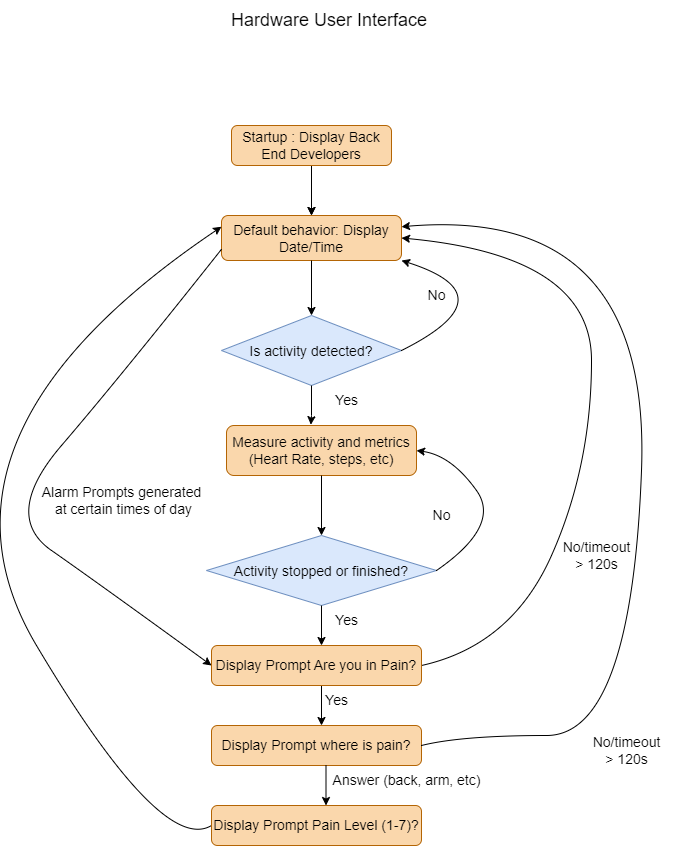
\includegraphics[width=1\textwidth]{HardwareUI_FSM}
		\caption{Flow chart model for Hardware UI (watch display)}
		\label{HardwareUI_FSM} 
	\end{center}
\end{figure}

\begin{figure}[H]
	\begin{center}
		 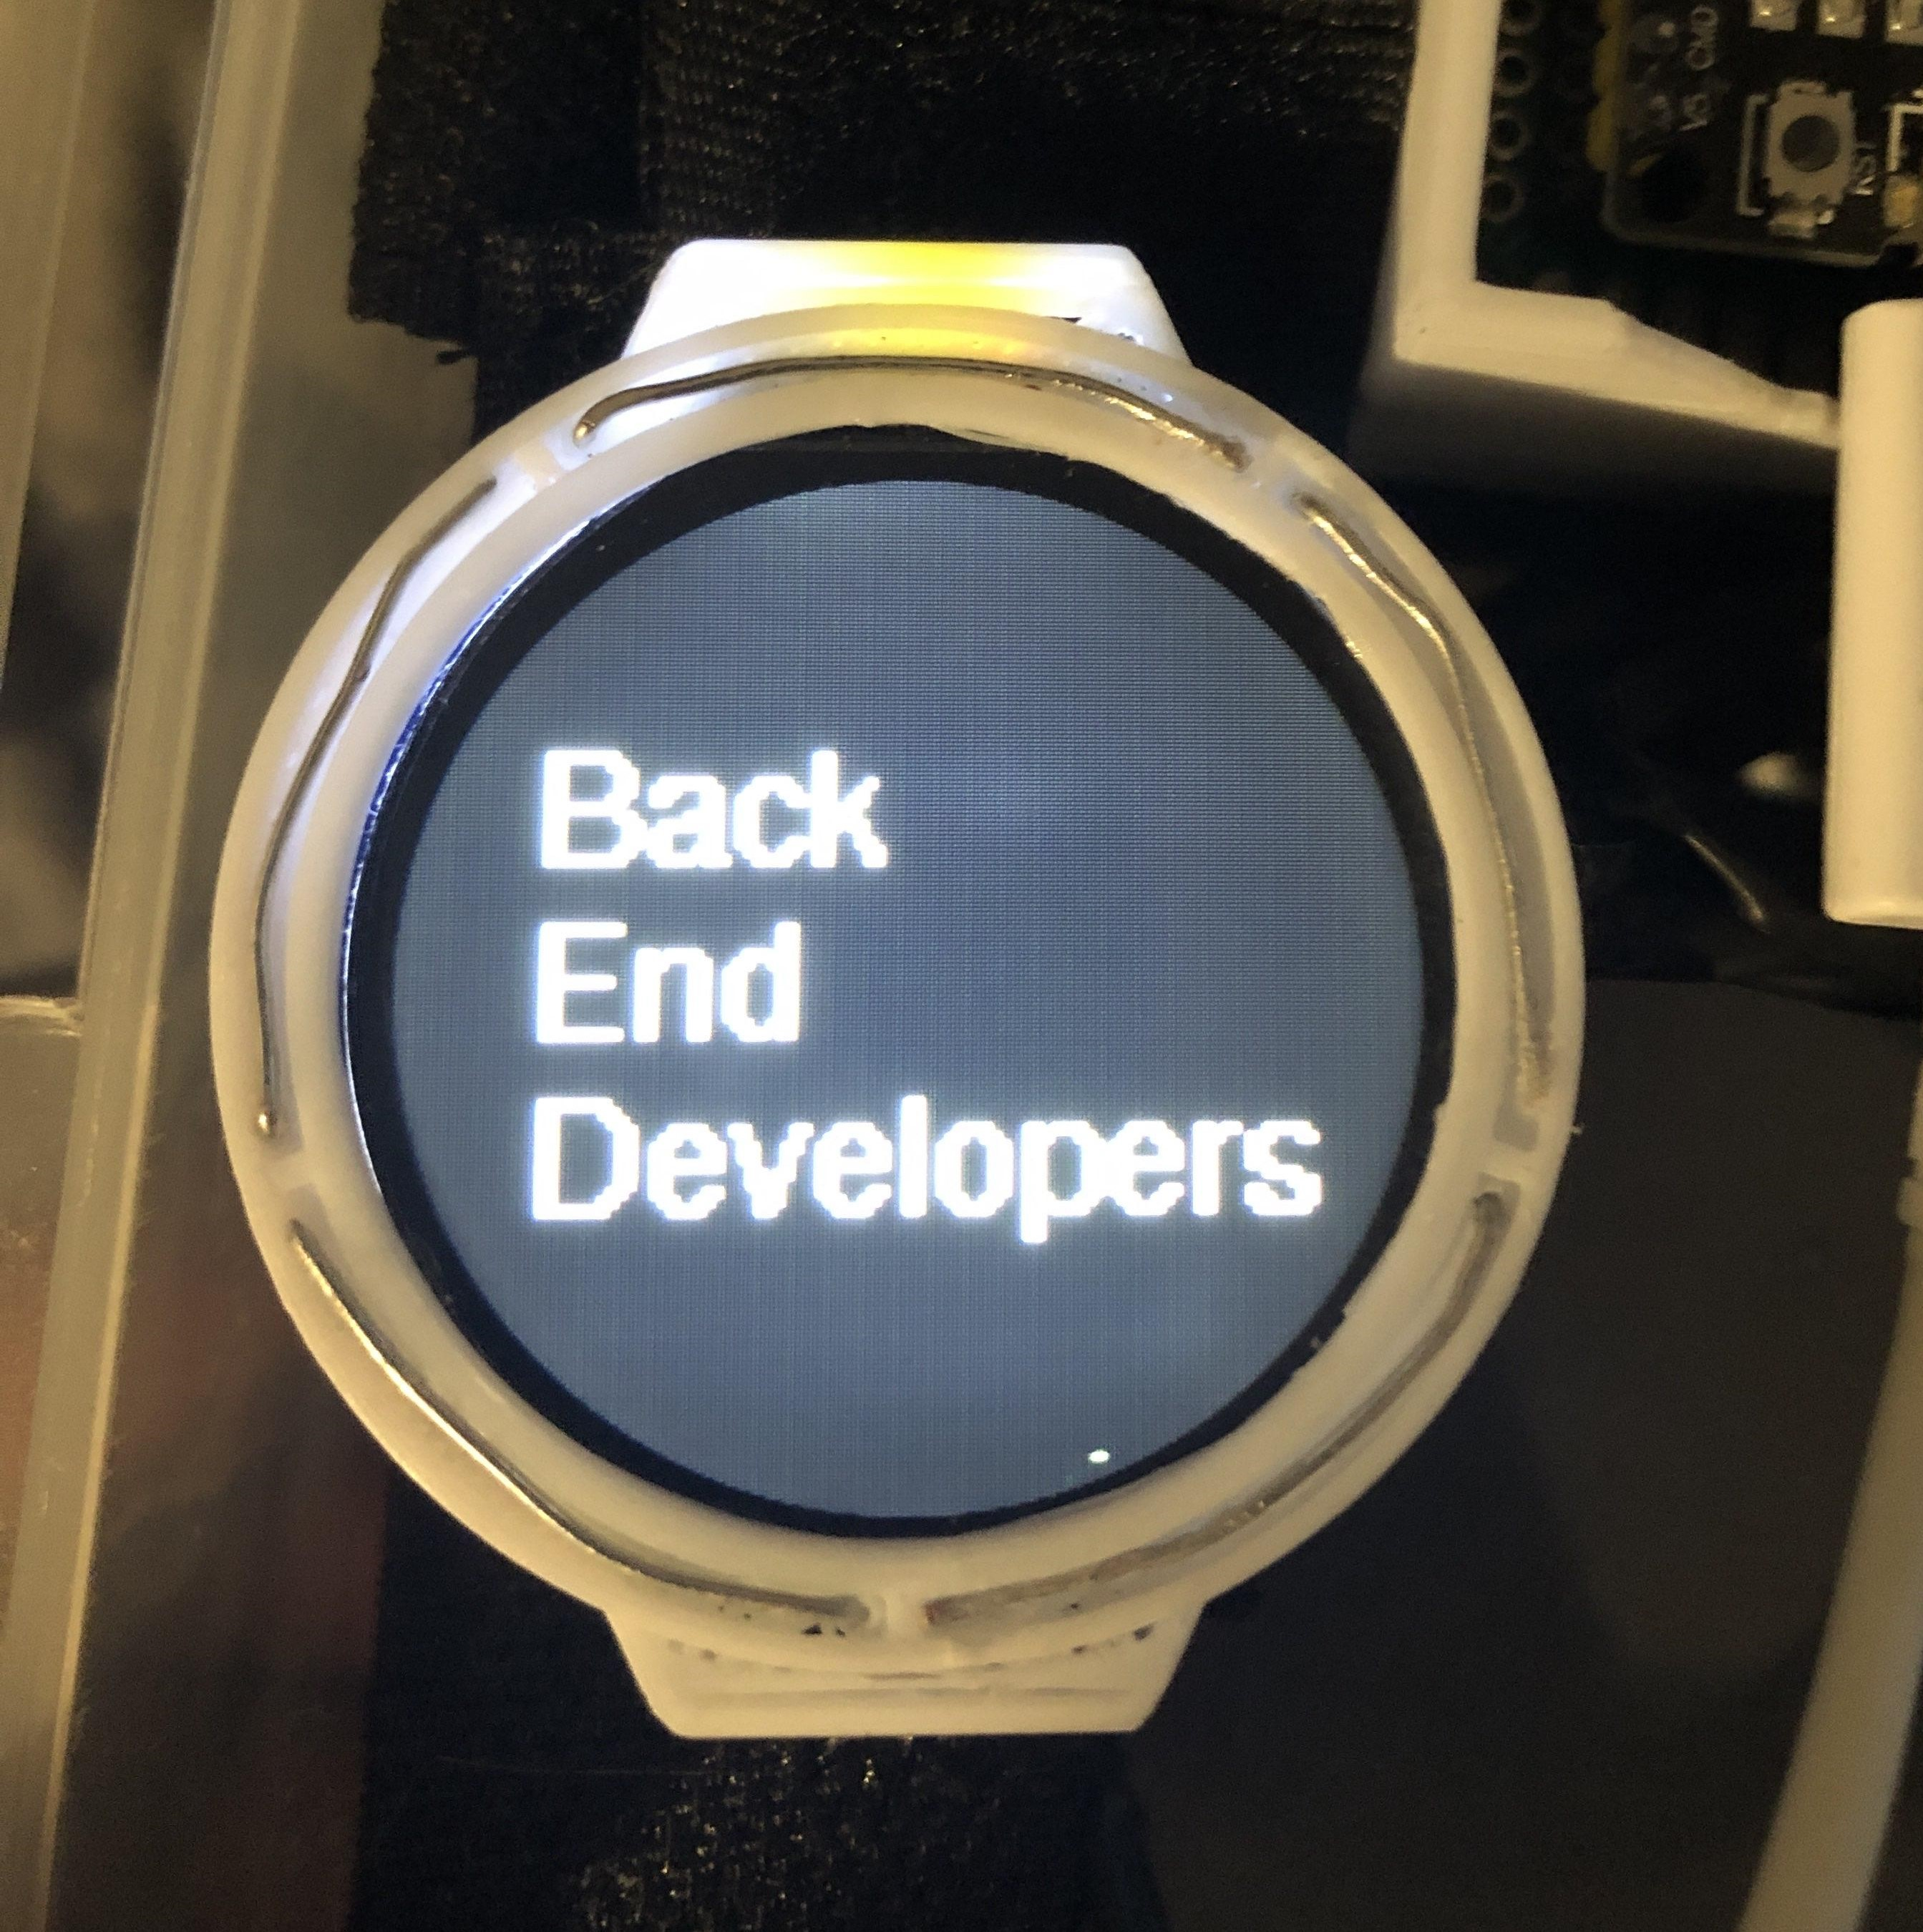
\includegraphics[width=0.5\textwidth]{BEDDisplay}
		\caption{Display on activity tracker at startup}
		\label{BEDDisplay} 
	\end{center}
\end{figure}

\begin{figure}[H]
	\begin{center}
		 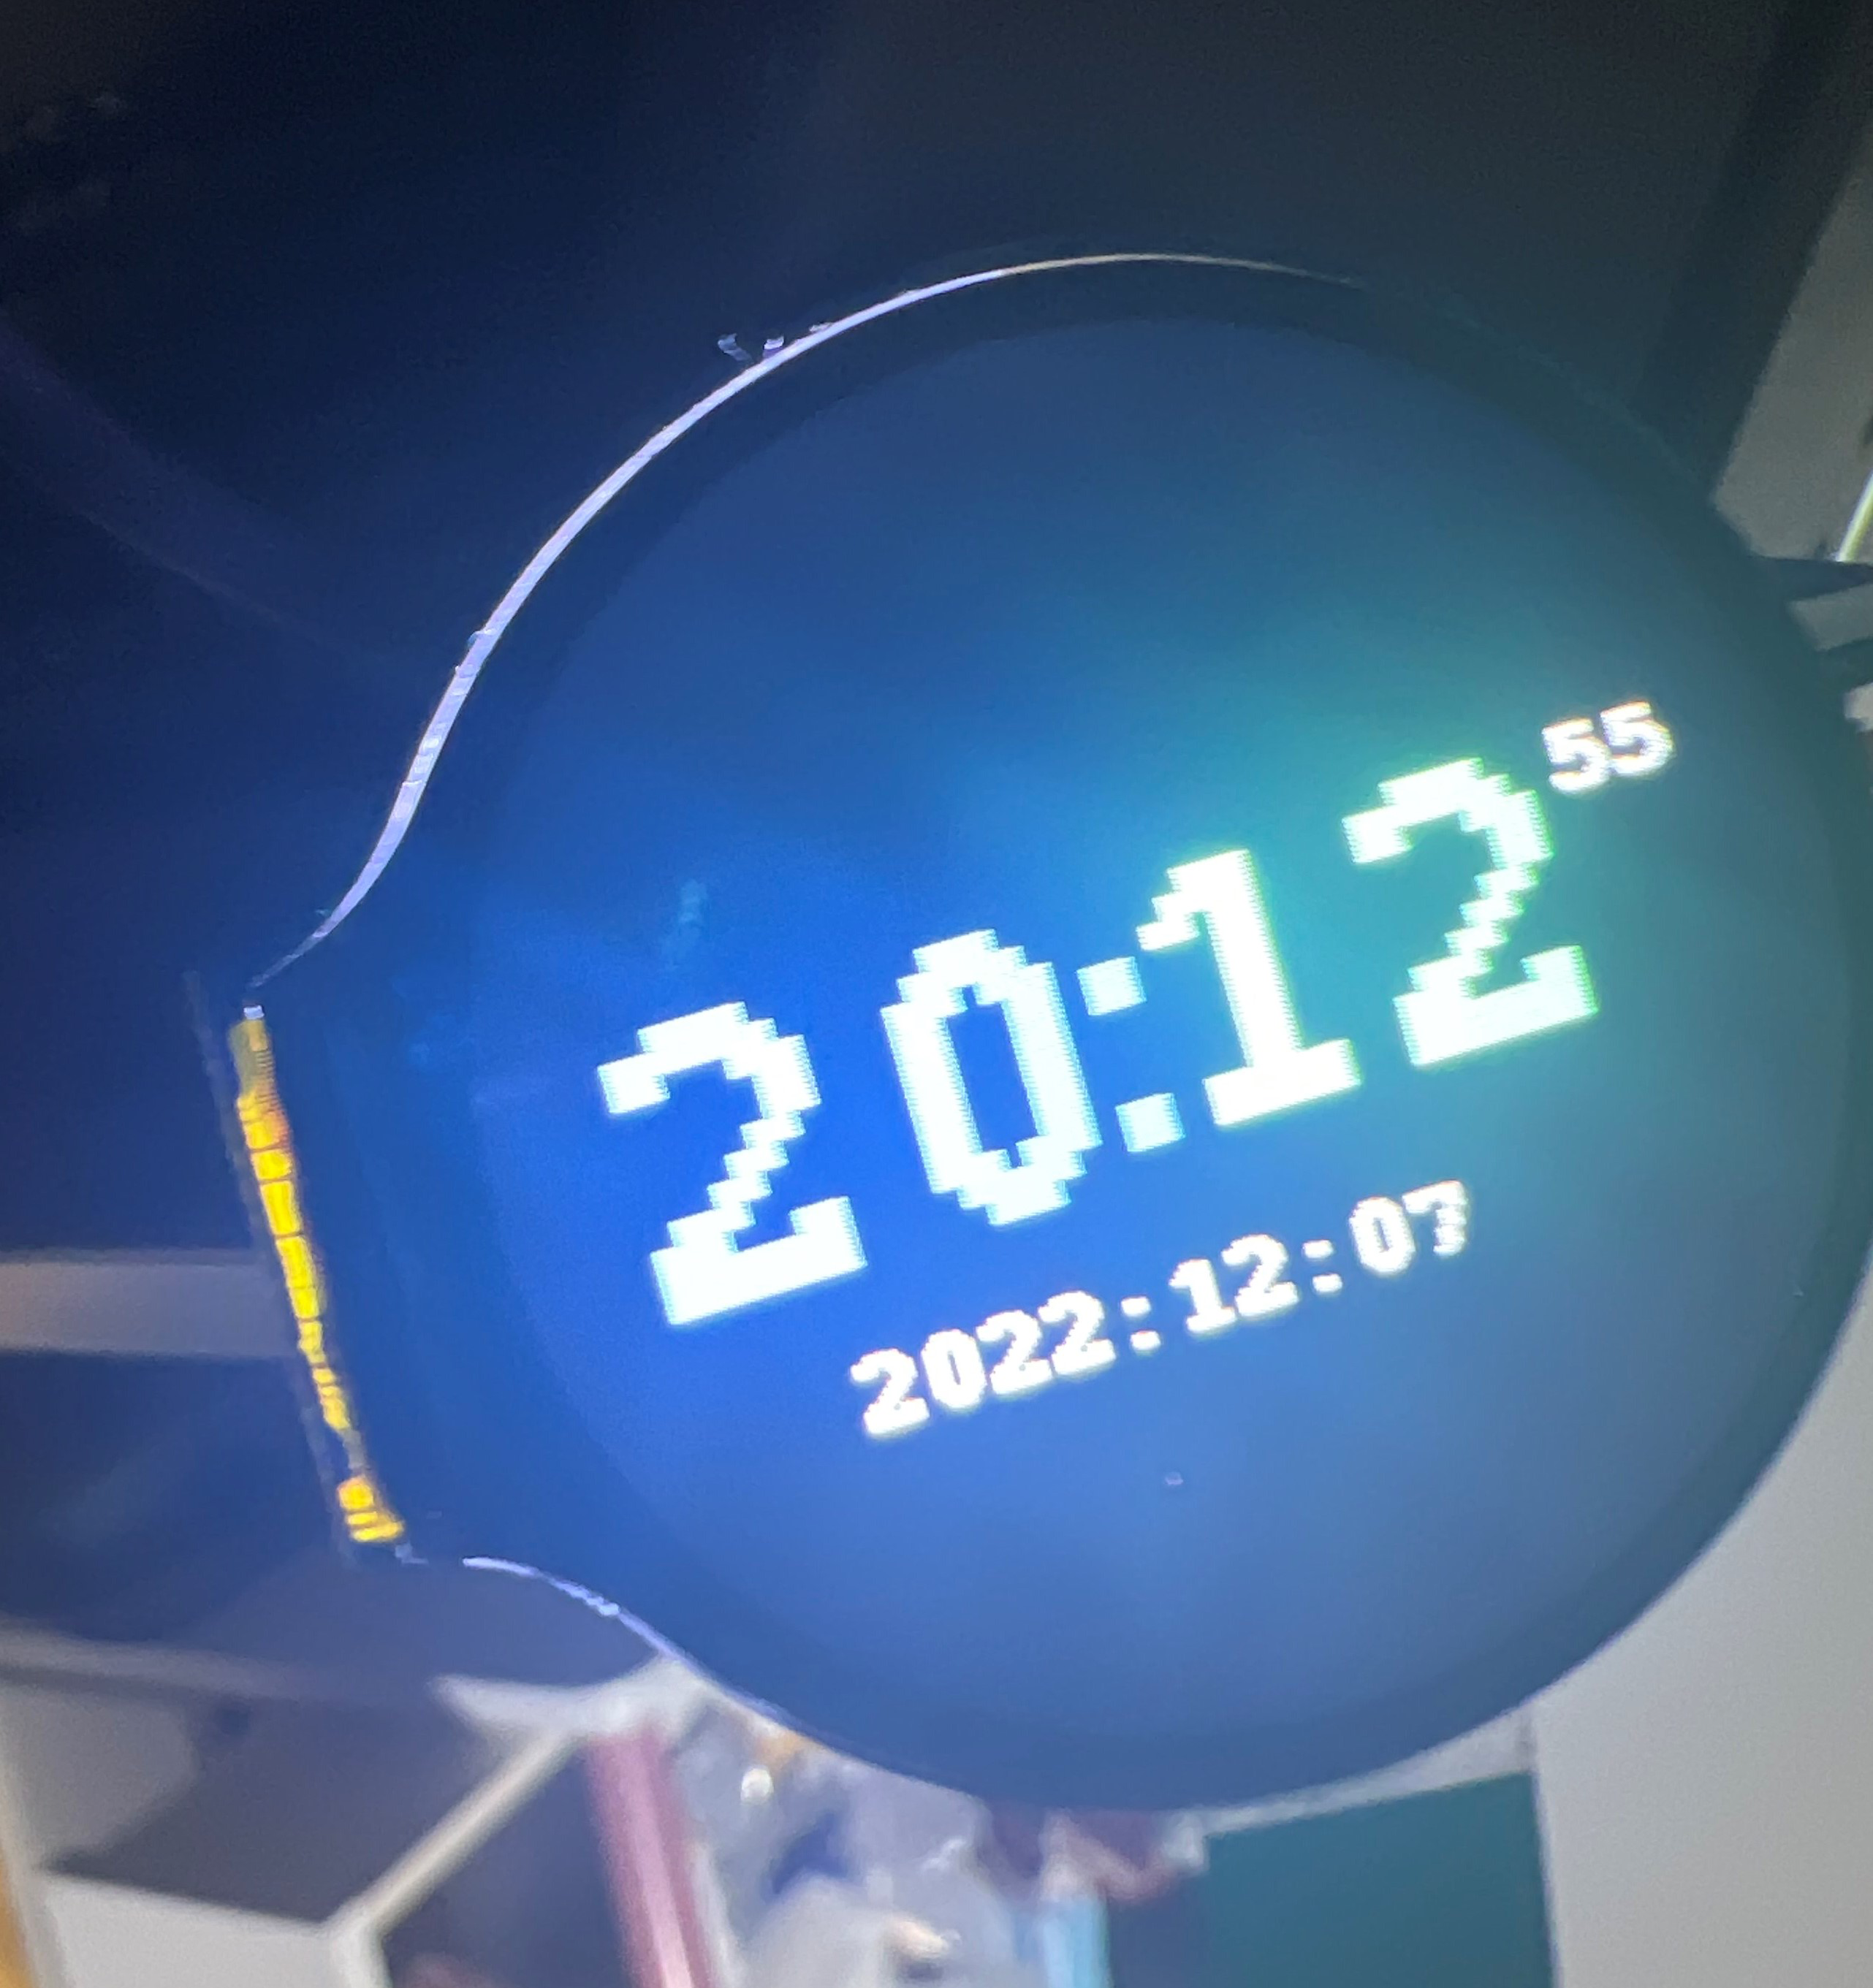
\includegraphics[width=0.5\textwidth]{DisplayTime}
		\caption{Display of date and time on activity tracker.}
		\label{DisplayTime} 
	\end{center}
\end{figure}
\newpage

\subsection{Software User Interface}

The software user interface will be used by the researcher for configuring the activity tracker. The interface will be on the host computer and will be able to store participant data, create new data and view records using encryption. The interface will also have authentication, and only the researcher will be able to log in. The following features are available on the software user interface:

\begin{table}[H]
	\begin{tabular}{|p{5cm}|p{10cm}|}
		 \hline
		 \textbf{Options on UI} & \textbf{Description}\\
		 \hline
		Main window & Main menu that leads to different windows when clicked.\\
		\hline
		 Connect to tracker  & Connects to SD card for device and shows status of connection.\\
		 \hline
		   Create records window & Creates new record for particpant and stores it in a database. A record can only be created if the correct username and password are provided. \\
		\hline 
		Records window & Participant records can be viewed in a tabular format and can be searched/filtered.\\
		\hline
		Data view window & Data stored on SD card can be viewed and filtered. Data can also be plotted using the graph button. For example: Heart rate vs time.\\
		\hline
	\end{tabular}
\caption{\label{Software User Interface}Components of Software UI}  
\end{table}

Below is an example of the Software User Interface for the Main window.
\begin{figure}[H]
	\begin{center}
		 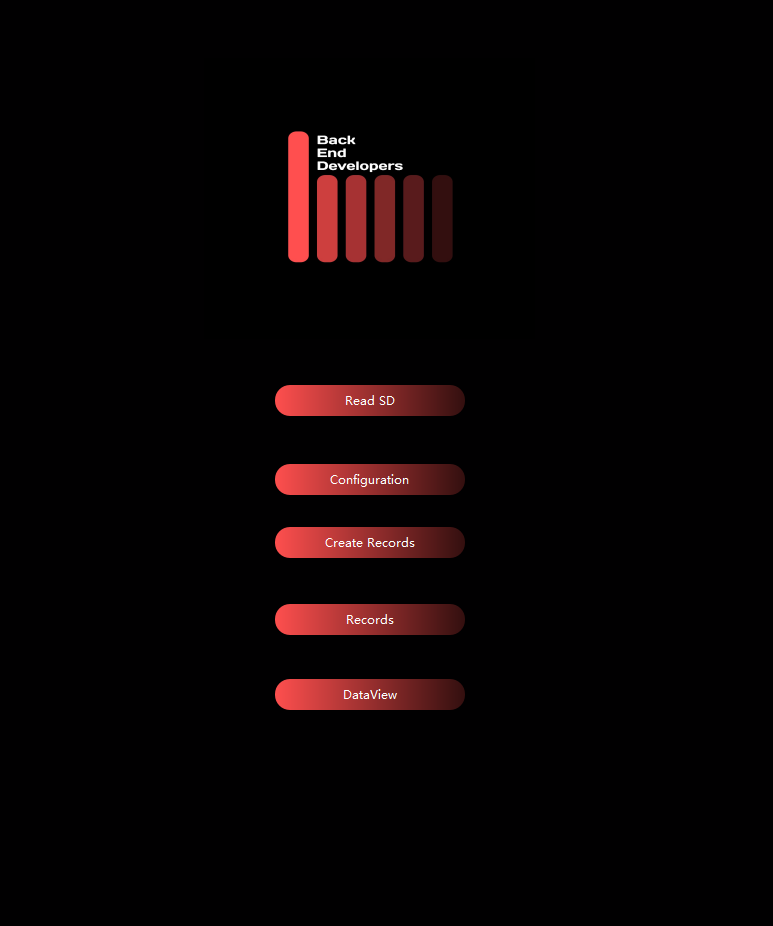
\includegraphics[width=0.4\textwidth]{MainWindow}
		\caption{Main Window for Software UI}
		\label{MainWindow} 
	\end{center}
\end{figure}

For more examples of the Software User Unterface, refer to Appendix \ref{Software_UI}.

\begin{figure}[H]
	\begin{center}
		 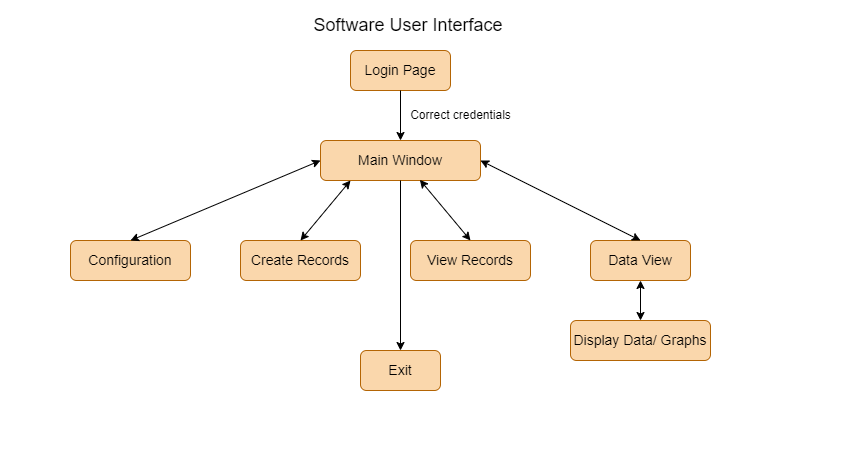
\includegraphics[width=1\textwidth]{SoftwareUI_FSM}
		\caption{Flow chart model of windows for Software UI}
		\label{SoftwareUI_FSM} 
	\end{center}
\end{figure}

\section{Design of Hardware}

The touch bezels shown in figures 7, 8, and 9 will be used as a bezel to navigate options on the activity tracker. The wires connected to each segment send a corresponding signal which can be used to navigate options and select a response.

\begin{figure}[H]
	\begin{center}
		 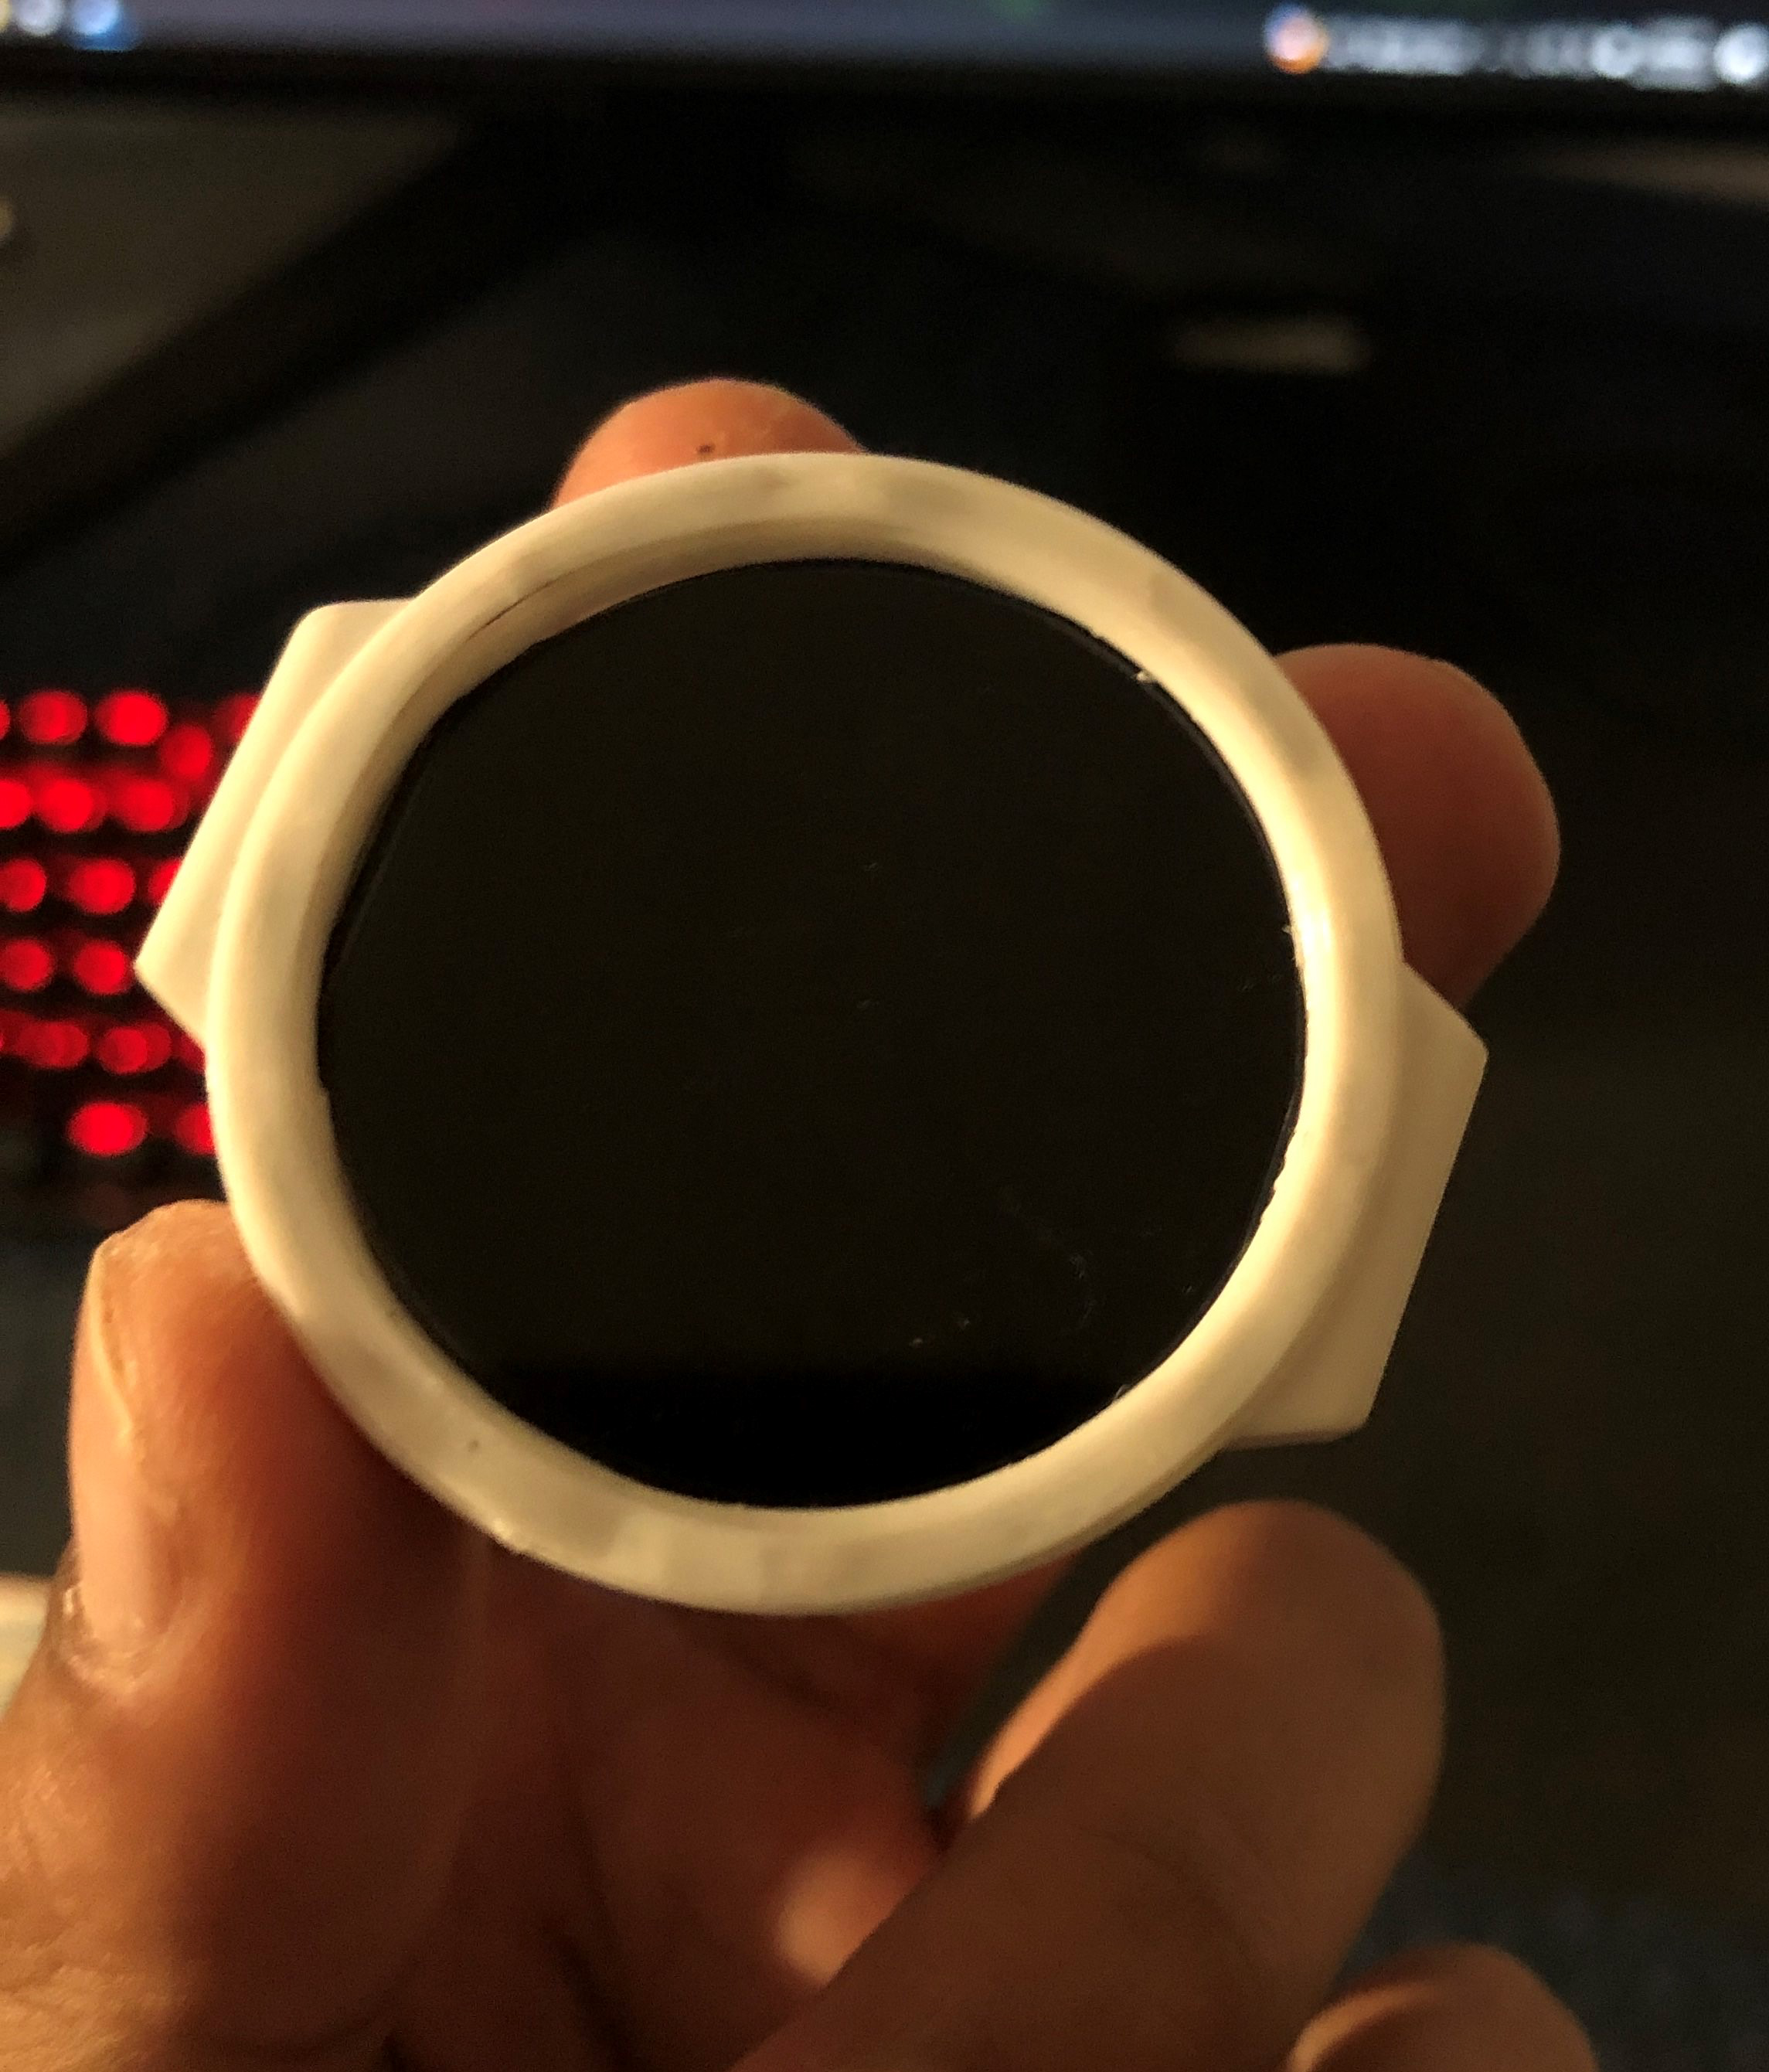
\includegraphics[width=0.3\textwidth]{DisplayCase}
		\caption{TFT Display with Custom 3D Printed Case}
		\label{DisplayCase} 
	\end{center}
\end{figure}

\begin{figure}[H]
	\begin{center}
		 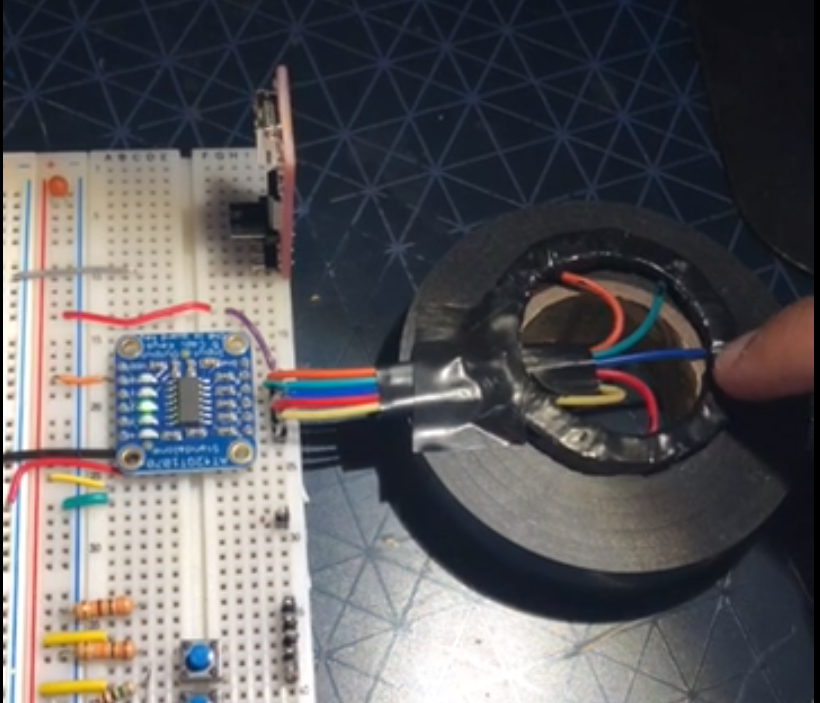
\includegraphics[width=0.6\textwidth]{TouchSensor}
		\caption{Circuit of Custom Built Reactive Touch Sensor}
		\label{TouchSensor} 
	\end{center}
\end{figure}

\begin{figure}[H]
	\begin{center}
		 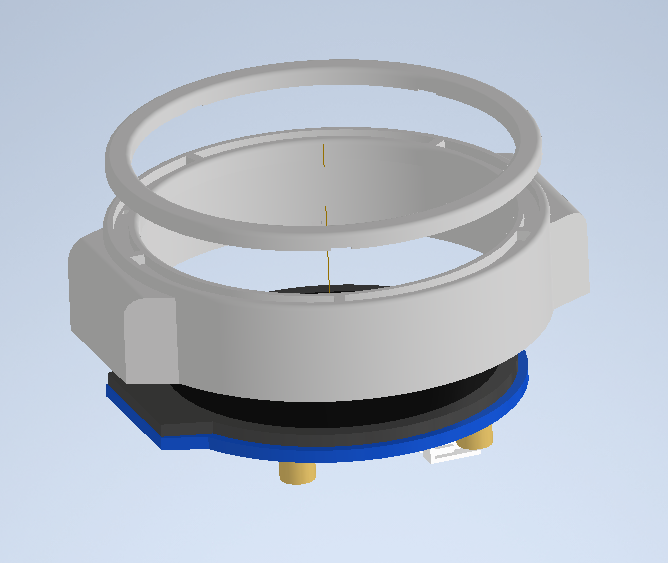
\includegraphics[width=0.5\textwidth]{WatchCAD}
		\caption{CAD Assembly of Touch Bezel, Display Case and TFT Display}
		\label{WatchCAD} 
	\end{center}
\end{figure}

\begin{figure}[H]
	\begin{center}
		 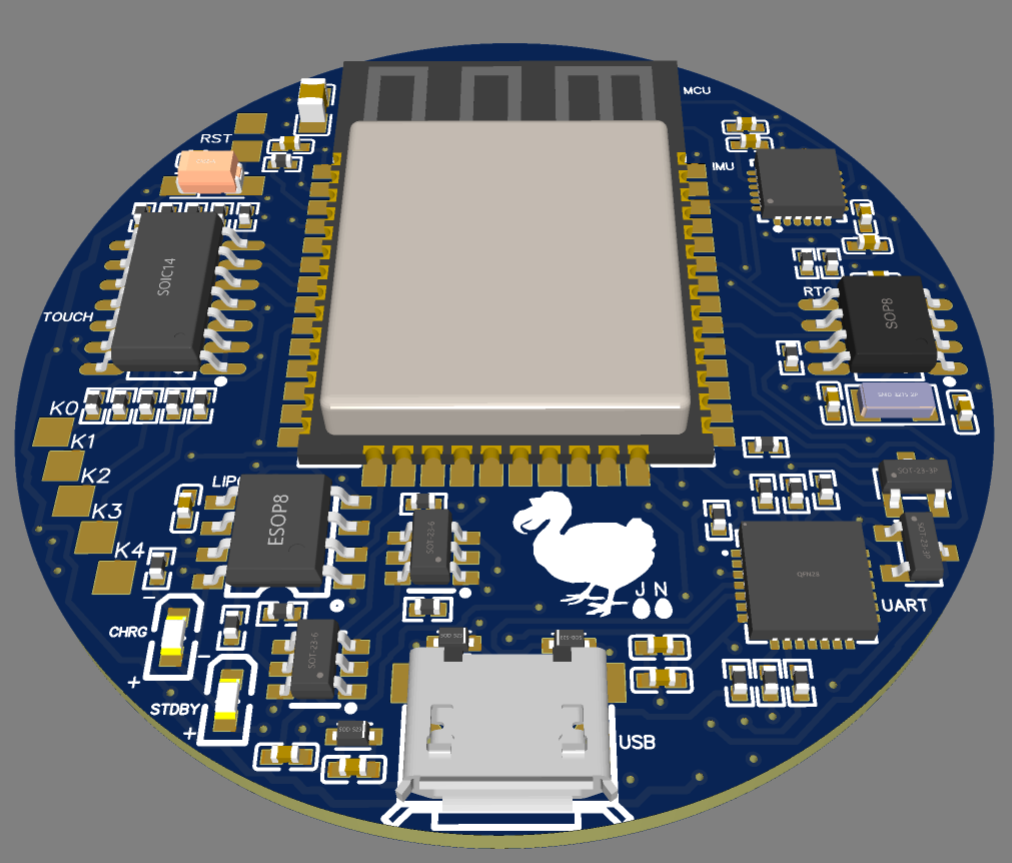
\includegraphics[width=0.5\textwidth]{PCBTOP}
		\caption{Top view of Custom PCB}
		\label{PCBTOP} 
	\end{center}
\end{figure}

\begin{figure}[H]
	\begin{center}
		 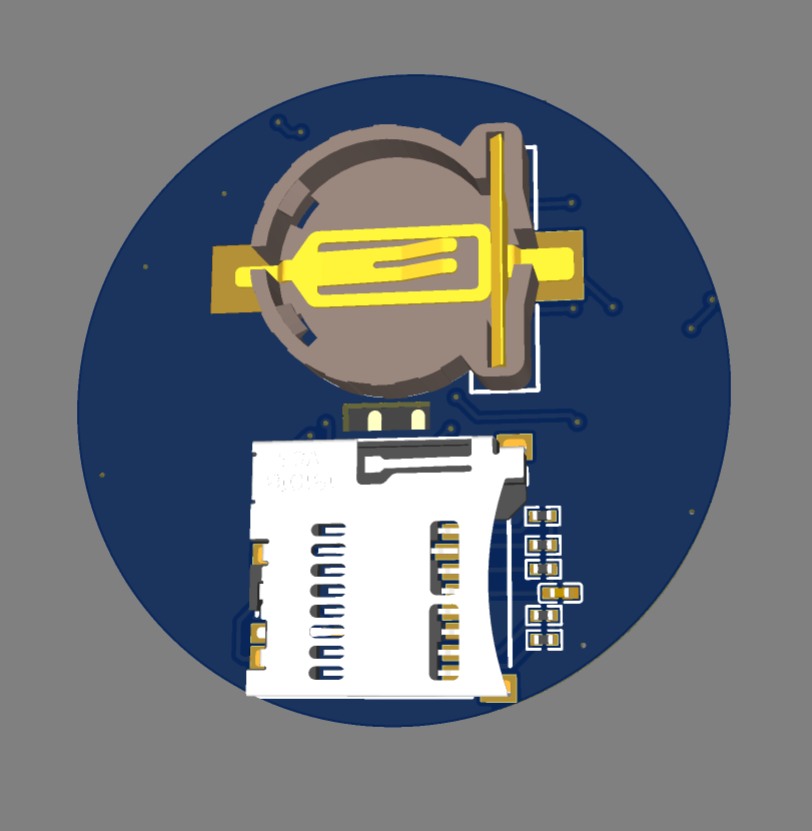
\includegraphics[width=0.5\textwidth]{PCBBOTTOM}
		\caption{Bottom view of Custom PCB}
		\label{PCBBOTTOM} 
	\end{center}
\end{figure}
\newpage
Refer to Appendix \ref{MechHardware} for individual CAD designs.\\

The following list of items will be custom designed and fabricated:
\begin{itemize}
\item{Custom PCB designed using \href{https://easyeda.com/}{Easy EDA} and fabricated using \href{https://jlcpcb.com/}{JLCPCB}}
\item{3D printed casing for TFT display/activity tracker.}
\item{Touch sensor (bezel) to navigate through activity tracker.}
\end{itemize}

Refer to table \ref{DesignHardware} in Appendix for detailed information on high-level hardware components used.

\section{Design of Electrical Components} \label{dEC}

The schematic/circuit diagrams shown below are used to generate the PCB layout. It consists of the following modules:
\begin{itemize}
\item ESP32-WROOM microcontroller
\item Touch sensor
\item Voltage regulator circuit
\item Battery protection circuit
\item RTC
\item MPU 6050 accelerometer
\item MicroSD card
\item LiPo battery
\item Pulse Sensor heartrate
\end{itemize}

\begin{figure}[H]
	\begin{center}
		 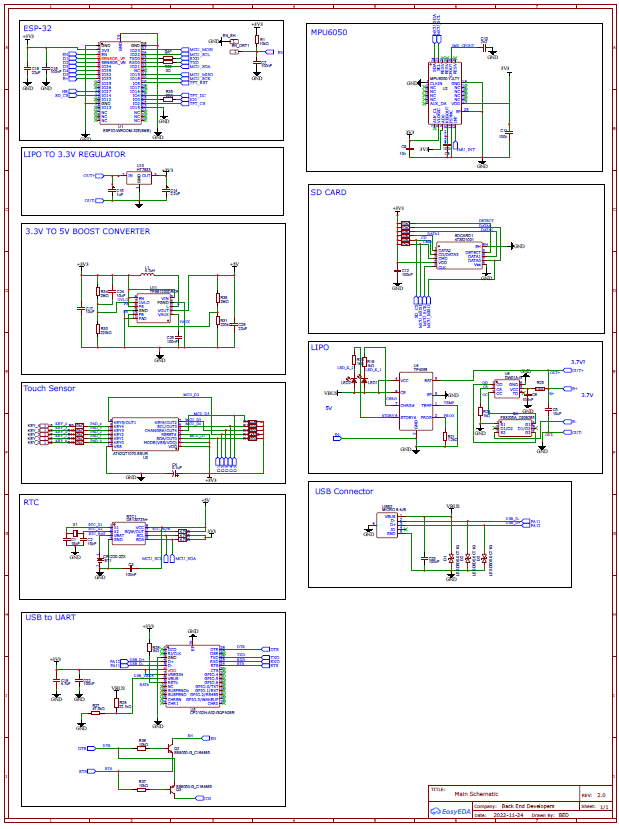
\includegraphics[width=1\textwidth]{Schematic}
		\caption{Schematic for PCB}
		\label{Schematic} 
	\end{center}
\end{figure}

The custom designed PCB is shown in figure 13.

\begin{figure}[H]
	\begin{center}
		 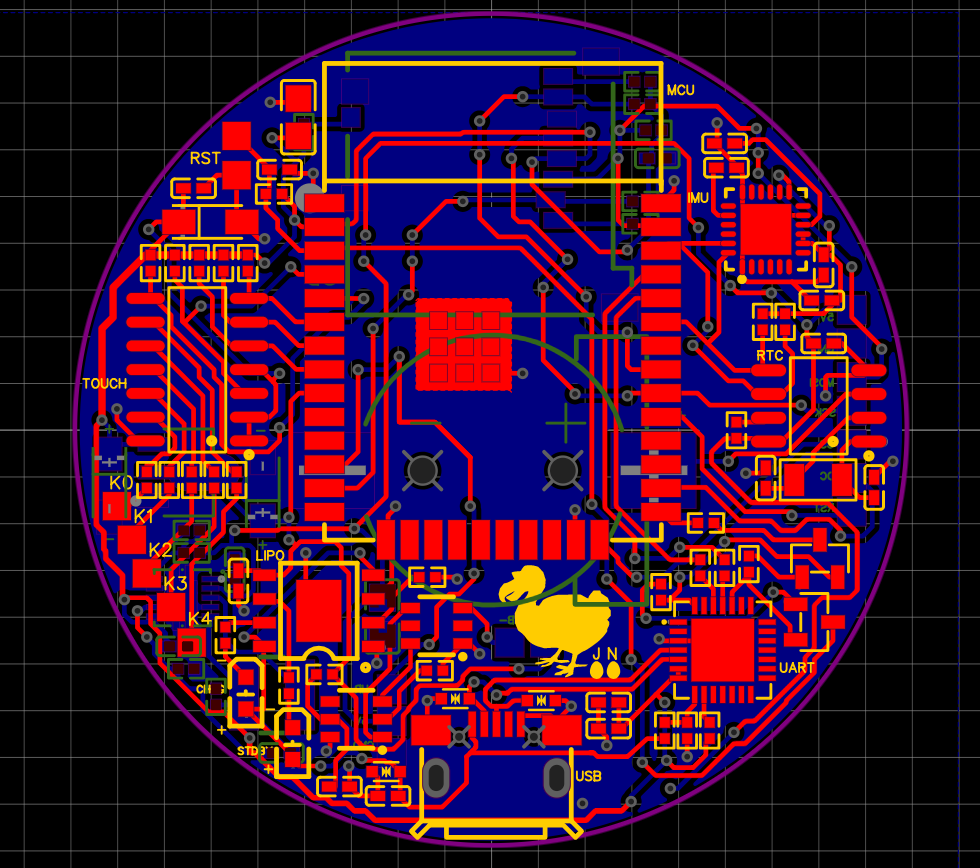
\includegraphics[width=0.75\textwidth]{Layout}
		\caption{Layout of PCB design}
		\label{Layout} 
	\end{center}
\end{figure}

Refer to table \ref{DesignElectrical} in Appendix for detailed information on electrical components (module-wise) used in the PCB design.

\section{Design of Communication Protocols}

There are two standard communication protocols that are used in the project, I2C and SPI. The following modules use I2C communication protocol:
\begin{itemize}
\item Code for RTC using I2C communication.
\item TFT display driver.
\item MPU 6050 driver.
\end{itemize}

The IO expander module uses SPI communication protocol.

\section{Timeline}

The following table outlines the project timeline for revision 0 demonstration:

\begin{table}[H]
\caption{\label{Timeline}Timeline of project Pt. 1}  
	\begin{tabular}{ | p{2.25cm} | p{4cm} |  p{3.5cm} | p{5.5cm} |}
		 \hline
		 \textbf{Timeline} & \textbf{Project Task} & \textbf{Member} & \textbf{Responsibilities}\\
		 \hline
		Dec 2022\newline- Jan 2023 & Front end software UI and functionality & Labeeb Zaker & Designing user friendly UI implementation. All UI design should be completed by the end of January.\\
		\hline
		Dec 2022\newline- Jan 2023 & Back end software UI and functionality & Jessica Bae & Implement authentication and encryption functionalities. Both funtionalities should be completed and cause no error. \\
		\hline
		Jan 2023 & Database management & Nish Shah & Implement database with software UI to read, store and write data. The UI should be able to fully interact with the database based on its implemented buttons.\\
		\hline
		Jan 2023 & UI and device connection & Nish Shah &Implement bluetooth connection and microSD connection between UI and device. MicroSD functionality should be completed. However, bluetooth functionality can be done after revision 0.\\
		\hline
		Dec 2022\newline- Jan 2023 & Accelerometer PCB schematic design & Anish Rangarajan & Implement schematics for accelerometer and gyroscope module in PCB. Schematic should be complete for PCB manufacturing.\\
		\hline
		Dec 2022\newline- Jan 2023 & microSD PCB schematic design & Jessica Bae & Implement the circuitry for microSD module in PCB. Schematic should be complete for PCB manufacturing.\\
		\hline
		Dec 2022\newline- Jan 2023 & LiPo battery PCB schematic design & Jonathan Hai & Implement the circuitry of LiPo battery module for PCB. Schematic should be complete for PCB manufacturing.\\
		\hline
	\end{tabular}
\end{table}

\begin{table}[H]
\caption{\label{Timeline}Timeline of project Pt.2}  
	\begin{tabular}{ | p{2.25cm} | p{4cm} |  p{3.5cm} | p{5.5cm} |}
		 \hline
		 \textbf{Timeline} & \textbf{Project Task} & \textbf{Member} & \textbf{Responsibilities}\\
		 \hline
		Dec 2022\newline - Jan 2023 & PCB layout design & Anish Rangarajan  & Implement PCB layout with proper routing. The layout should be complete for PCB manufacturing.\\
		\hline
		Nov 2022 & Display driver& Labeeb Zaker & Display driver for the device should be able to handle displaying time and prompt, as required per revision 0.\\
		\hline
		Nov 2022 & Device frame CAD model & Anish Rangarajan & CAD models for device frame.\\
		\hline
		 February 1 2023\newline- Feb 6 2023 & Integration of all sensor modules & Jonathan Hai, Oliver Foote & Integrate all sensors and systems and create test benches to check correct functionality.\\
		\hline
			Jan 2023 \newline-March 2023 & PCB testing  & Jessica Bae, Oliver Foote & Performing system-wide testing on PCB based on \href{https://github.com/zakerl/Capstone_Project/blob/main/docs/VnVPlan/VnVPlan.pdf}{VnVPlan} \\
		\hline
		Continuous untill April 2023 & Documentation & All team members & Complete all documentation.\\
		\hline
	\end{tabular}
\end{table}


% \bibliographystyle {plainnat}
% \bibliography{../../../refs/References}

\newpage{}

\appendix

\section{Software Interface}
\label{Software_UI}

\begin{figure}[H]
	\begin{center}
		 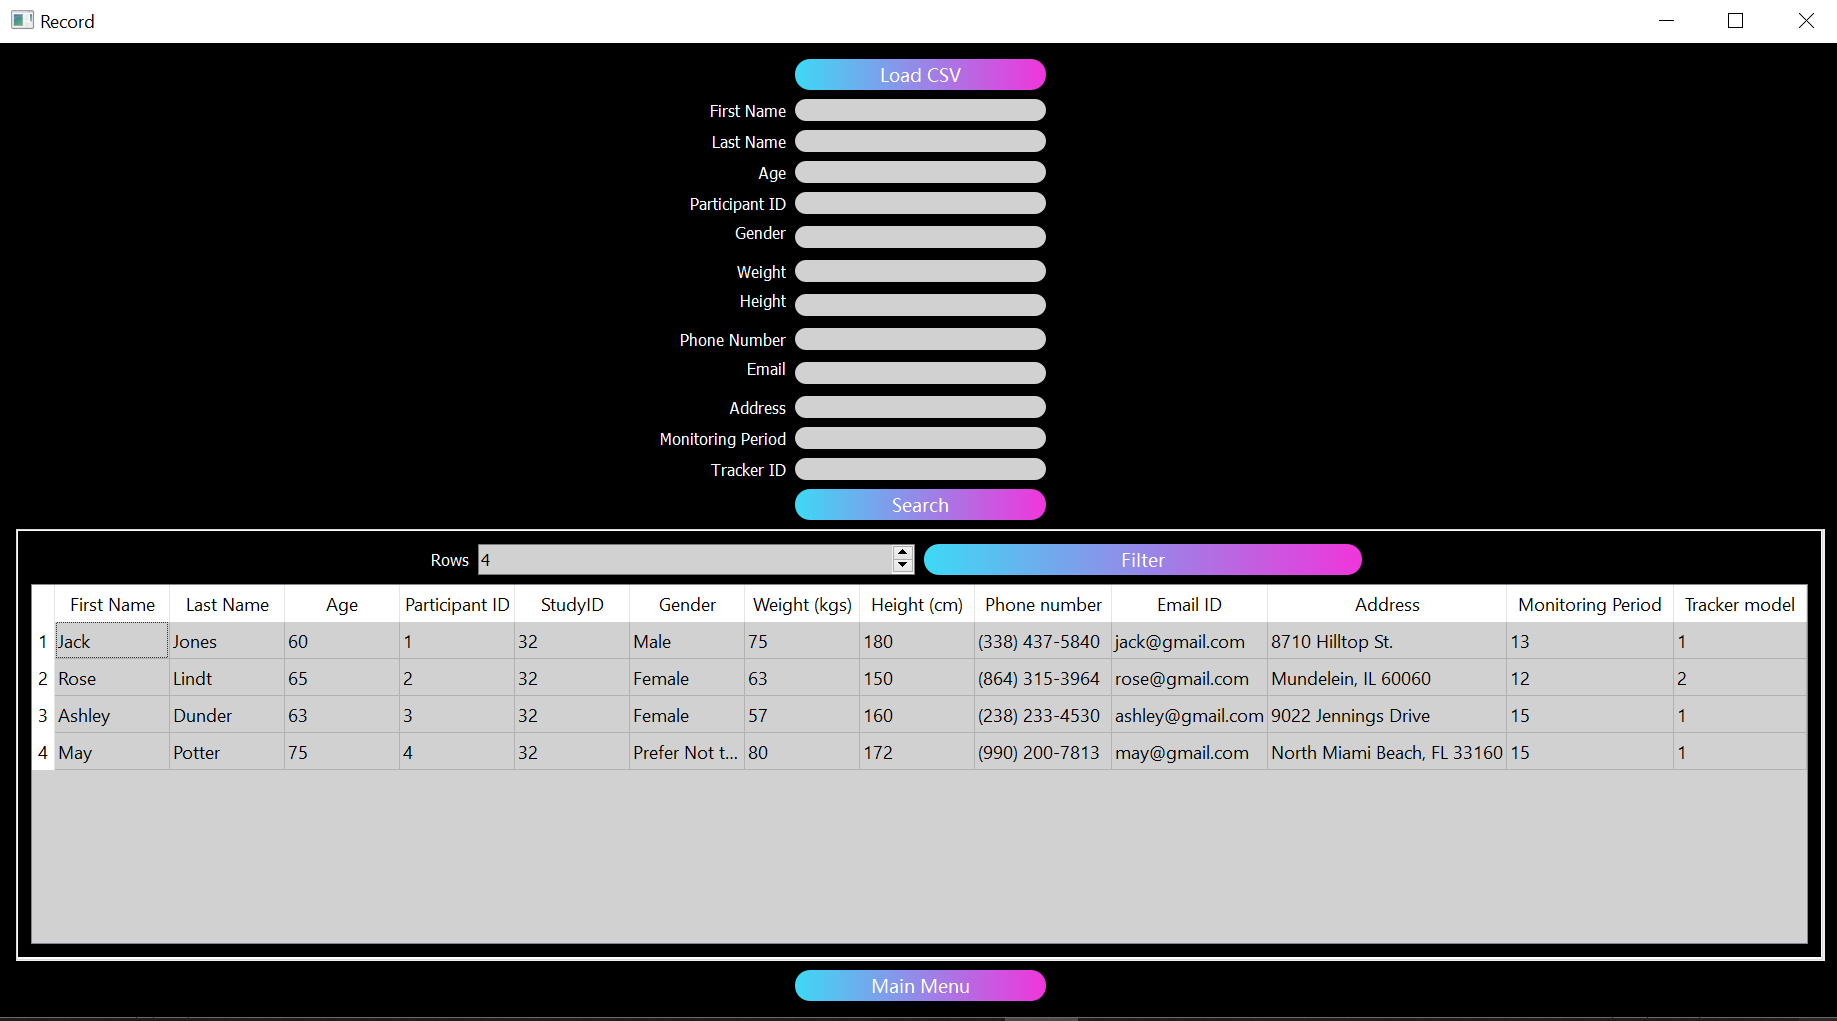
\includegraphics[width=0.9\textwidth]{Record}
		\caption{Record Window}
		\label{Record} 
	\end{center}
\end{figure}

\begin{figure}[H]
	\begin{center}
		 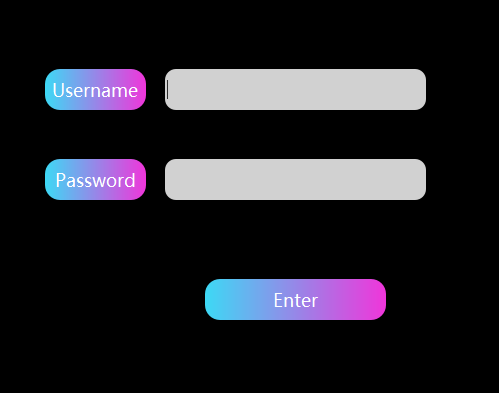
\includegraphics[width=0.4\textwidth]{login}
		\caption{Login Page}
		\label{Login} 
	\end{center}
\end{figure}

\begin{figure}[H]
	\begin{center}
		 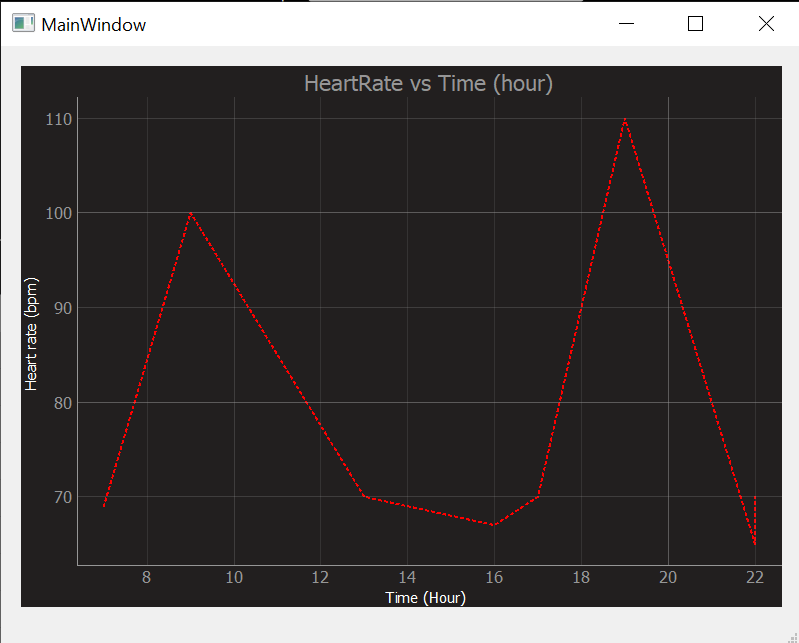
\includegraphics[width=0.8\textwidth]{Graph}
		\caption{Generated Graph for Heart Rate vs Time}
		\label{Graph} 
	\end{center}
\end{figure}
\section{Hardware Interface}
\label{MechHardware}

\begin{figure}[H]
	\begin{center}
		 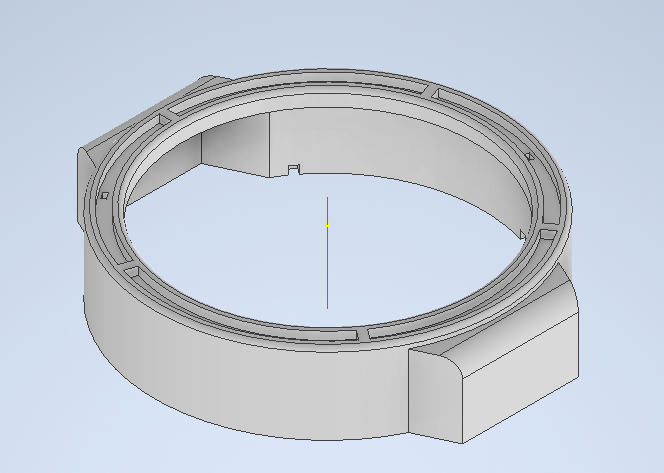
\includegraphics[width=0.5\textwidth]{DisplayCaseCAD}
		\caption{CAD Model of Case for TFT Display}
		\label{DisplayCaseCAD} 
	\end{center}
\end{figure}

\begin{figure}[H]
	\begin{center}
		 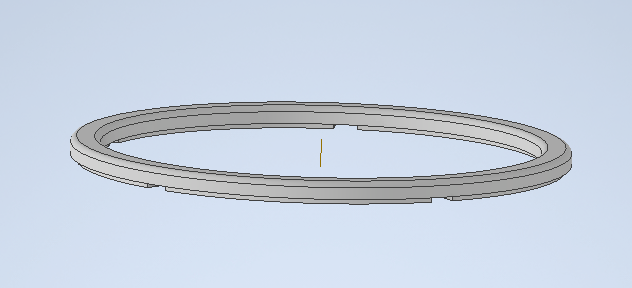
\includegraphics[width=0.5\textwidth]{BezelCAD}
		\caption{CAD Model of Touch Sensor (Bezel)}
		\label{BezelCAD} 
	\end{center}
\end{figure}

\begin{figure}[H]
	\begin{center}
		 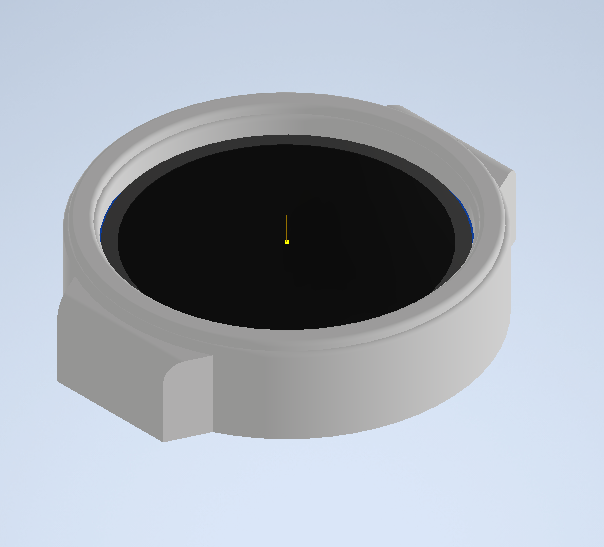
\includegraphics[width=0.5\textwidth]{WatchCAD2}
		\caption{CAD Model of Watch Assembled}
		\label{WatchCAD2} 
	\end{center}
\end{figure}

\begin{figure}[H]
	\begin{center}
		 \includegraphics[width=1\textwidth]{Hardware}
		\caption{Overall Hardware Design}
		\label{Hardware} 
	\end{center}
\end{figure}

\begin{table}[H]
	\begin{tabularx}{1.05\textwidth} { 
		  | >{\centering\arraybackslash}X 
		  | >{\centering\arraybackslash}X 
		  | >{\centering\arraybackslash}X 
		  | >{\centering\arraybackslash}X | }
		 \hline
		 \textbf{Hardware Component} & \textbf{Description}\\
		 \hline
		Custom PCB & Custom PCB designed to fit in activity tracker.  \\
		\hline 
		Touch bezels & Custom 3D printed touch bezels for user interaction with the activity tracker.\\
		\hline
		Outer casing for TFT display & Designed using Autodesk Inventor and 3D printed. \\
		\hline 
		AT42QT1070-SSUR & Off-shelf microchip for capacitive touch sensors, used in touch sensor schematic.\\
		\hline
		 MPU 6050 & Off-shelf accelerometer and gyroscope.\\
		\hline
		 ESP32-WROOM  & Off-shelf microcontroller for activity tracker.\\
		 \hline
		   DS1307 RTC & Off-shelf real time clock. \\
		\hline
		Waveshare 1.28 LCD-192 display & Off-shelf TFT display used in activity tracker. \\
		\hline 
		Pulse Sensor & Off-shelf plug and play heart rate sensor.\\
		\hline 
		LiPo battery & Generic off-shelf LiPo battery used for smart watches.  \\
		\hline 
		TP4056 Li-Ion BMS & Off-shelf constant-current/constant-voltage linear charge for battery, used in LiPo schematic.\\
		\hline
		DW01A-G & Off-shelf battery protection IC  to protect battery from overcharge, used in LiPo schematic.\\
		\hline
		USB type-B charger & Generic off-shelf usb to type-B charger to charge device. \\
		\hline 
		MicroSD card & Standard off-shelf microSD card. \\
		\hline
		SDCARD connector 473521001& Off-shelf microSD connector. \\
		\hline 
		Watch straps & Generic watch-straps for strapping device onto the wrist. \\
		\hline 
	\end{tabularx}
\caption{\label{DesignHardware}Components of Hardware Design}  
\end{table}

\section{Electrical Components}
\begin{table}[H]
	\begin{tabular}{| p{4cm} | p{12cm} |}
		 \hline
		 \textbf{Module} & \textbf{Electrical component}\\
		\hline
		 MPU 6050  & \begin{itemize}
						\item{Capacitors (2nF, 10nF, 100nF)}
						\item{Resistors (4.7k ohms)}
					\end{itemize}\\
		\hline
		 Touch sensor  & \begin{itemize}
						\item{Capacitors (0.1uF)}
						\item{Resistors (470 ohms, 10k ohms)}
					\end{itemize}\\
		 \hline
		 RTC  & \begin{itemize}
						\item{Capacitors (15pF, 100nF)}
						\item{Resistors (4.7k ohms)}
					\end{itemize}\\
		 \hline
		 microSD Card & \begin{itemize}
						\item{Capacitors (100nF)}
						\item{Resistors (10k ohms)}
					\end{itemize}\\
		 \hline
		 LiPo Battery & \begin{itemize}
						\item{Capacitors (100nF, 10uF)}
						\item{Resistors (100 ohms, 1k ohms, 1.2k ohms)}
						\item{FS8205 MOSFET}
					\end{itemize}\\
		 \hline
	\end{tabular}
\caption{\label{DesignElectrical}Electrical Components of modules from PCB schematic}  
\end{table}

\section{Communication Protocols}

Bluetooth communication was implemented using socket programming in Python. The library \href{https://github.com/pybluez/pybluez}{PyBluez} was used to initialize sockets and to establish the connection between the host computer and the device. The host computer directly connects to the device securely using a pin, and data is grabbed from the onboard microSD card and transferred to the computer using bluetooth-serial communication. Bluetooth was also used to send various data to the device including configuration files, formatting SD card, and resetting device.

\section{Reflection}

The information in this section will be used to evaluate the team members on the
graduate attribute of Problem Analysis and Design.  Please answer the following questions:

\begin{enumerate}
  \item \textit{What are the limitations of your solution?  Put another way, given
  unlimited resources, what could you do to make the project better? }(LO\_ProbSolutions)\\

This is a difficult question to answer. Given unlimited resources, the Back End Developers would have many more options available in fundamental design, and may have pursued a different design altogether --- however going forward with this question it is assumed that this question refers to the current design on hand.\\

There are many forms of "resources" that have to be managed during an engineering project. Cost, time, testing opportunities, and many more constraining factors can be considered resources. Let us consider cost and time, as those have the largest and most obvious impacts on the project.\\

Given an unlimited budget, the face of the EMAnator likely would have been a touchscreen, as the cost of a touchscreen was prohibitively high and we had to find a workaround using nearby capacitive touch sensors instead. In addition, we would have kept ordering test PCBs of our designs as we iterated through different versions. This would have allowed us to test individual components and wiring routes as we constructed the final design. As cost is limited, we have to finish the whole design first, and proceed to order a very limited number of test PCBs on which we must test all aspects of our design. We will then revise the design to compensate for issues found on the test boards, order the final set, and pray that they work as intended. We would also consider adding an operating system to the device to make it "smart". Currently our device has a very limited number of functions that fit tightly into our requirements. An OS would enable us to expand the functionality of our device beyond its current borders.\\

If the design could have taken place over an infinite amount of time, there are additional possibilities that we could consider. Primarily, we could investigate using and shrinking down a more powerful microcontroller. Currently, the type of microcontroller that we can use is extremely limited in its capabilities. However if we wish to upgrade to a more powerful one (e.g. a Raspberry Pi), we would have to place a large number of auxiliary components necessary for the functioning of the more powerful (and more needy) processor. This would have taken a large amount of time; as finding reasonable space on a PCB and routing components like these is notoriously time consuming.\\

Obviously there are many new and exciting possibilities for this project should certain resources be unlimited. But overall, we are satisfied with the design that we have made given the constraints that have been placed on us. Should we decide to continue developing this device past the capstone course, we may return to these options at a certain point.\\

  \item \textit{Give a brief overview of other design solutions you considered.  What
  are the benefits and tradeoffs of those other designs compared with the chosen
  design?  From all the potential options, why did you select documented design?}
  (LO\_Explores)\\

During the initial phases of the design process, we encouraged each other to throw around as many design ideas as we could. Here is a short list of a few we considered, along with a few of their pros and cons:\\
\begin{itemize}
\item Anklet Activity Tracker\\
	Pros:
	\begin{itemize}
		\item Discreet and unobstructive to daily activities.
		\item High-quality data available regarding motion of legs (steps, jumps, falls, etc.).
	\end{itemize}
	Cons:
	\begin{itemize}
		\item Difficult to reach for people with difficulty bending over.
		\item If designed poorly, can potentially look like a prison ankle monitor.
		\item Difficult for a user to read any data displayed on a screen on the anklet.
	\end{itemize}
\item Waist-Mounted Activity Tracker\\
	Pros:
	\begin{itemize}
		\item Being close to the core of the user, the maximum weight of the device can be greatly increased.
		\item Easy access to those with difficulty bending over, or with other movement related issues.
	\end{itemize}
	Cons:
	\begin{itemize}
		\item Located in a hard-to-hide location, and may get in the way of reaching below the waist.
		\item Incompatible with certain clothing.
	\end{itemize}
\item Bracelet Activity Tracker\\
	Pros:
	\begin{itemize}
		\item Extremely discreet.
		\item High-quality data available regarding motion of arms (walker use, exercise, etc.).
		\item Not obstructive to daily activities.
	\end{itemize}
	Cons:
	\begin{itemize}
		\item Interacting with a small-surface area bracelet may be difficult for those with movement issues.
		\item Small size reduces battery capacity options.
	\end{itemize}
\item Full Body Suit Tracker\\
	Pros:
	\begin{itemize}
		\item Highest fidelity data possible, collecting data from every point on the body.
		\item Difficult to misplace.
	\end{itemize}
	Cons:
	\begin{itemize}
		\item Prohibitively expensive.
		\item Easy to damage.
		\item Many people would be uncomfortable wearing a full sized-body suit during all their daily activities.
	\end{itemize}
\item Mobile App \\
	Pros:
	\begin{itemize}
		\item Inexpensive.
		\item Flexible; meaning we can modify it according to new requirements whenever necessary.
		\item Many are already extremely familiar with activity tracking apps; onboarding process will not be difficult.
		\item Can be linked to off-the-shelf smartwatches with fantastic activity collecting technology.
	\end{itemize}
	Cons:
	\begin{itemize}
		\item Not a mechatronics solution.
	\end{itemize}
\end{itemize}
Why did we pursue the smart-watch solution? For two very important reasons; end-user familiarity and end-user acceptability.\\

The other solutions that we could have proceeded with may have met all the functional requirements and many of the nonfunctional requirements that we specified, but many of them are unfamiliar and possibly confusing to the end user. For example, having to wear a box around one's waist is likely a novel and strange experience to any user, and could make them uncomfortable with using the device in general. In addition, most people have worn a watch before, and are very familiar with their operations. This makes the process of learning how to use the watch simpler and more intuitive.\\

A smart-watch was also deemed the most acceptable solution to an end user. It would be difficult to convince anyone to wear a sensor covered spandex suit everywhere they went in their daily life, for a period of up to 14 days. A watch is familiar, socially acceptable, and much less embarrassing than wearing a full bodied suit similar to the figure below.

\end{enumerate}

\begin{figure}[H]
	\begin{center}
		 \includegraphics[width=1\textwidth]{Pink}
		\caption{Example of Someone Experiencing a Full Body Suit}
		\label{Pink} 
	\end{center}
\end{figure}

\end{document}